\documentclass[tikz]{standalone}
\usetikzlibrary{automata,positioning}
\begin{document}
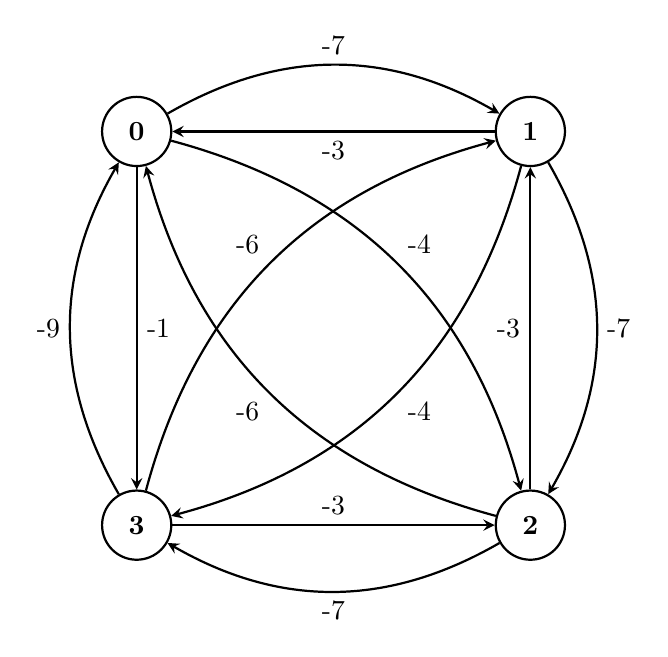
\begin{tikzpicture}[>=stealth,node distance=2cm, on grid, auto, thick, initial text=] 
	\node[state] (0) {\textbf{0}}; 
	\node[state] (1) [right=5cm of 0] {\textbf{1}};
	\node[state] (2) [below=5cm of 1] {\textbf{2}};
	\node[state] (3) [below=5cm of 0] {\textbf{3}};
	
	\path[->]		(0) edge [bend left] node {-7} (1)
					(1) edge [bend left] node {-7} (2)
					(2) edge [bend left] node {-7} (3)
					(3) edge [bend left] node {-9} (0)
					
					(0) edge node {-1} (3)
					(3) edge node {-3} (2)
					(2) edge node {-3} (1)
					(1) edge node {-3} (0)
					
					(0) edge [bend left] node {-4} (2)
					(2) edge [bend left] node {-6} (0)
					(1) edge [bend left] node {-4} (3)
					(3) edge [bend left] node {-6} (1);
\end{tikzpicture}
\end{document}